\documentclass[10pt,twoside,a4paper,brazil]{abntex2}
\usepackage[utf8]{inputenc}
\usepackage[brazil]{babel}
\usepackage[T1]{fontenc}
\usepackage{amsmath}
\usepackage{amsfonts}
\usepackage{amssymb}
\usepackage{graphicx}
\usepackage{hyperref}
\usepackage{float}
\usepackage[num]{abntex2cite}
\usepackage{indentfirst}

\graphicspath{{./img/}}

\titulo{Pontos de Lagrange}

\autor{Benjamin Garcia de Figueiredo -- 9783741\\Eduardo Amâncio Barbosa Oliveira -- 	9783592\\Henrique de Almeida Tórtura -- 9762702\\Jonathas Queiroz Ribeiro Moraes -- 9762661\\Lucas Lopes Costa -- 9783716\\Octávio da Motta -- 9863458\\Pedro Antônio Soares de Alcântara -- 9783629\\Wilson Santana Martins -- 9791476} % TODO: Checar forma mais eficiente e esteticamente melhor de listar os contribuidores
\local{São Carlos, Brasil}
\data{2017}

\instituicao{
   Universidade de São Paulo -- USP
   \par
   Instituto de Física de São Carlos -- IFSC
}


\tipotrabalho{Artigo Científico}

\preambulo{Trabalho apresentado no curso de Mecânica Clássica, ministrado pelo professor Roberto Nicolau Onody, no Instituto de Física de São Carlos da Universidade de São Paulo, como parte do processo avaliativo da disciplina.}

\makeatletter

\hypersetup{
   pdftitle={\@title},
   pdfauthor={\@author},
   pdfsubject={\imprimirpreambulo},
   pdfkeywords={{Pontos de Lagrange}, {Mecânica Clássica}, {Estabilidade}, {Simulação Computacional}}, % TODO
   pdfcreator={LaTeX with abnTeX2},
   colorlinks=true,
   linkcolor=blue,
   citecolor=blue,
   urlcolor=blue
}

\makeatother
\begin{document}
   \imprimircapa
   
   \imprimirfolhaderosto   
   
   \tableofcontents

	 \newpage
	 
   \begin{resumo}
      Este trabalho visa expor e discutir questões acerca da concepção dos denominados pontos de Lagrange, que surgem naturalmente na análise de um problema de três corpos como uma extensão do problema de Kepler circular, apoiando-se inclusive nos textos precursores na obtenção dos mesmos, como publicações originais de Euler e Lagrange, sobre os três primeiros pontos e a inclusão dos dois últimos, respectivamente. Estrutura-se com o objetivo de desenvolver uma interpretação física e fenomenológica, partindo do problema restrito de dois corpos de onde obtivemos as funções horárias das componentes, as quais nos permitem escolher um referencial rotacional estacionário em relação a ambas. Extende-se o modelo adicionando um terceiro corpo consideravelmente menos massivo que os anteriores, e neste panorama de interação ternário, calculamos as coordenadas dos pontos de Lagrange através de métodos que permeiam o curso de graduação de Mecânica Clássica. Outrossim, uma investigação mais minuciosa dos pontos nos leva a conclusão de que dois deles são estáveis, equanto os demais são instáveis, exibindo seus autovalores. Isso posto, um exemplo de aplicação é apresentado: o modelo de Roche para sistemas binários de estrelas. Nele, modela-se uma estrela hidrodinamicamente como um ponto contendo toda sua massa cercado por um envelope de massa nula. Além disso, apresentamos uma simulação computacional de partículas, escrita em C++11, baseada em um integrador numérico Runge-Kutta de quarta ordem para integração das equações newtonianas de movimento das partículas situadas nos pontos em que há interesse, a fim de que adquiríssemos informações relevantes para a caracterização dos pontos lagrangianos e constatações de suas estabilidades. O referido problema, por muito tempo, se apresentou como paradigma da física teórica, justificando, portanto, a realização dessa obra.

      \vspace{\onelineskip}
      \noindent
      \textbf{Palavras-chave}: Pontos de Lagrange, Mecânica Clássica, Estabilidade, Simulação Computacional
   \end{resumo}

   \chapter{Introdução}
      Placeholder

      
   \chapter{Teoria}
      \section{Gravitação e o problema de n-corpos}

Dois corpos massivos ocupando posições diferentes no espaço sofrem uma atração proporcional ao produto de suas massas e ao inverso do quadrado de sua distância mútua no sentido que os une. Isso é descrito pelo potencial,

\begin{equation}
    \label{eq:gravitacaouniversal}
    U(\mathbf{r}_1 - \mathbf{r}_2) = -\frac{Gm_1m_2}{||\mathbf{r}_1 - \mathbf{r}_2||}
\end{equation}

Mas o espaço é homogêneo, e o movimento do sistema pode depender apenas das posições relativas dos objetos. Isso motiva que se defina

\begin{align}
    \mathbf{R} &= \mathbf{r}_1 - \mathbf{r}_2 && \mu = \frac{m_1m_2}{m_1 + m_2}
\end{align}

e as equações de movimento se reduzem a

\begin{equation}
    \mu \ddot{\mathbf{R}} = -\frac{\partial U}{\partial \mathbf{R}}
\end{equation}

e como

\begin{align}
    \mathbf{r}_1 &= \mathbf{r}_{CM} + \frac{m_2}{m_1 + m_2}\mathbf{R} && \mathbf{r}_2 = \mathbf{r}_{CM} - \frac{m_1}{m_1 + m_2}\mathbf{R}
\end{align}

conclui-se que num referencial baricêntrico o problema de dois corpos é simplesmente o problema de força central, que é resolvido, pela mudança de variável $u = \frac{1}{r}$ num sistema de coordenadas polar perpendicular ao momento angular $\mathbf{L}$ (que é conservado), através da equação de Binet,

\begin{equation}
    \label{eq:binet}
    \frac{d^2u}{d\theta^2} + u = -\frac{\mu}{\mathbf{L}^2}F\left(\frac{1}{u}\right).
\end{equation}

Assim, obtem-se a trajetória e, com algum esforço, a evolução temporal do sistema. Sistemas de dois corpos ou de um corpo (caso limite para um dos corpos muito mais massivo que o outro) admitem, em situações de energia negativa, órbitas elípticas

\begin{equation}
    r(\theta) = \frac{a(1 - e^2)}{1 + e\cos (\theta - \theta_0)}.
\end{equation}

Sistemas gravitacionais de mais de dois corpos são, por outro lado, impossíveis de se resolver analiticamente no caso geral. Num sistema de $n$ partículas interagindo entre si exclusivamente gravitacionalmente, a equação de movimento da $i$-ésima partícula é 

\begin{equation}
    \ddot{\mathbf{r}}_i=-\sum_{\substack{j=1\\j \neq i}}^{n} \frac{Gm_j(\mathbf{r}_j - \mathbf{r}_i)}{||\mathbf{r}_j - \mathbf{r}_i||^3}.
\end{equation} 

Trata-se de uma situação consideravelmente mais complexa que a de poucos corpos, uma vez que não há mais conservação de momento angular de cada partícula, a possibilidade de colisões gera singularidades nas soluções e o desacoplamento das equações não é possível. Apesar disso, é possível analisar e resolver sistemas de $n$-corpos, especialmente na presença de restrições e aproximações adequadas.

Os pontos de Lagrange emergem naturalmente na análise de um problema de três corpos como uma extensão do problema de Kepler circular: Sendo $R$ a distância entre dois objetos de massas $m_1$ e $m_2$, tomamos um referencial baricêntrico que gira com velocidade angular constante $\omega$ igual à orbital

\begin{equation}
    \omega^2 = \frac{G(m_1 + m_2)}{R^3}
\end{equation}

Caso um corpo estacionário de massa $m$ seja inserido nesse sistema, preservando coplanaridade, observar-se-á agindo sobre ele uma força centrífuga (e, caso se movimentasse, também uma força de Coriolis. Garantidamente não há força de Euler nesse tratamento), de forma que o potencial efetivo se torna

\begin{equation}
    U_{ef}(\mathbf{r}) = - \frac{Gmm_i}{||\mathbf{r} - \mathbf{r}_1||} - \frac{Gmm_i}{||\mathbf{r} - \mathbf{r}_2||} - \frac{1}{2}\mathbf{r}^2\omega^2
\end{equation}

e escolhendo um ponto no espaço $\mathbf{r_0} \neq \mathbf{r}_i$, observamos que o conjunto

\begin{align} 
    \Lambda &= \{\mathbf{r} | U_{ef}(\mathbf{r}) \geq U_{ef}(\mathbf{r_0}) - \epsilon\}
\end{align}

é, para $\epsilon > 0$, fechado e, como $U_{eff}$ tende a $-\infty$ para $||\mathbf{r}||$ grande, limitado e portanto compacto. Assim, a função atinge nele um máximo $\mathbf{r_M}$. $\mathbf{r_M}$ está necessariamente contido no interior de $\Lambda$, já que $U_{ef}(\mathbf{r_M}) \geq U_{ef}(\mathbf{r_0})$. Pela diferenciabilidade de $U_{ef}$ o ponto é estacionário: um objeto de massa negligível nesse ponto realizará movimento circular uniforme ao redor do centro de massa do sistema.

Para fins práticos, entretanto, existência é insatisfatória, mas motiva o cálculo desses pontos, dentre outros pontos estacionários do potencial efetivo, que serão justamente os pontos de Lagrange.

\section{Problema restrito de 2 corpos}

Nas coordenadas do centro de massa, podemos escrever:

\begin{align}
    \mathbf{r}_1 &=  \frac{m_2}{m_1 + m_2}\mathbf{R} && \mathbf{r}_2 = - \frac{m_1}{m_1 + m_2}\mathbf{R}
\end{align}

E, analisando a força gravitacional sobre um dos corpos:

\begin{equation}
\mathbf{F} = m_1\mathbf{\ddot{r}}_1 = \mu\mathbf{\ddot{R}} = -\frac{Gm_1m_2}{R^3}\mathbf{R} \label{dia}
\end{equation}

E note que ocorre exatamente o mesmo para o corpo 2. Podemos escrever a (\ref{dia}) como:

\begin{equation}
\mathbf{\ddot{R}} + \frac{G(m_1+m_2)}{R^3}\mathbf{{R}} = 0 \label{dif}
\end{equation}

E, uma vez resolvida a (\ref{dif}), obtêm-se as funções horárias de ambas as partículas. Nos restringiremos aqui ao caso em que a distância entre os 2 corpos é constante. Nesse caso, a equação se torna simplesmente uma equação de oscilador harmônico em cada uma das coordenadas, e $\mathbf{R}$
realiza um movimento circular uniforme cuja frequência é dada por:

\begin{equation}
\omega^2 = \frac{G(m_1+m_2)}{R^3} \label{kepi}
\end{equation}

\section{Dedução dos pontos de Lagrange}

Interessa-nos agora analisar uma extensão do problema anterior, adicionando no sistema um terceiro corpo, de massa $m<<m_1,m_2$, de maneira que ele não perturbe a órbita original nem desloque o centro de massa do sistema. 

\begin{figure}[H]
\centering
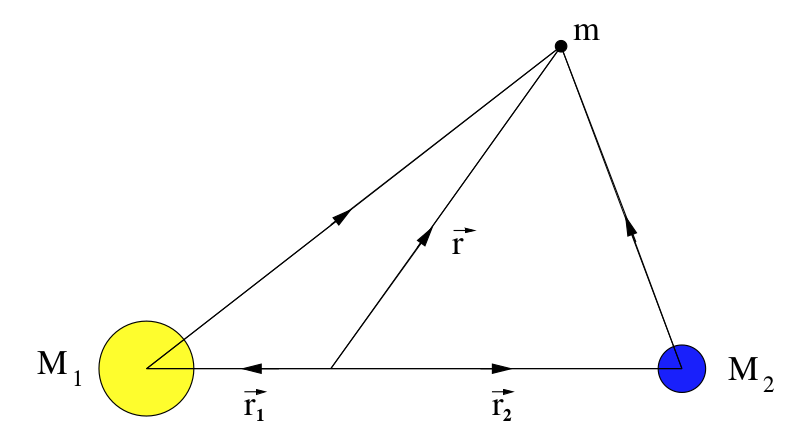
\includegraphics[scale = 0.5]{3_corpos.png}
\caption{Problema restrito de 3 corpos.}
\end{figure}


Temos que as forças atuantes sobre ele são:

\begin{align}
\mathbf{F_1} = -\frac{Gm_1m}{|\mathbf{r}-\mathbf{r_1}|^3}(\mathbf{r}-\mathbf{r_1}) && \mathbf{F_2} = -\frac{Gm_2m}{|\mathbf{r}-\mathbf{r_2}|^3}(\mathbf{r}-\mathbf{r_2})
\end{align}

Nessas condições, chamamos de pontos de Lagrange os pontos que permitem uma órbita estacionária para o terceiro corpo, mantendo constantes as distâncias entre os três corpos.

Como $\mathbf{r_1}$ e $\mathbf{r_2}$ são funções do tempo, torna-se mais conveniente tratar do problema num referencial baricêntrico que gira com velocidade angular constante $\omega$. Nesse caso, devemos levar em consideração as forças de inércia:

\begin{equation}
\mathbf{F_{IN}} = -m\boldsymbol{\omega} \times (\boldsymbol{\omega} \times \mathbf{r}) -2m(\mathbf{\omega} \times \mathbf{\dot{r}}) 
\end{equation}

Onde o primeiro termo corresponde à força centrífuga e o segundo, à força de Coriolis. Note que nesse referencial, os pontos de Lagrange correspondem a pontos de equilíbrio estático, nos quais a força resultante (incluindo as forças de inércia) é nula. Para uma solução estática, devemos, é claro, ter que $\mathbf{\dot{r}}=0$. Escolhendo coordenadas cartesianas convenientemente alinhadas, temos:

\begin{eqnarray}
\boldsymbol{\omega} & = & \omega\mathbf{\hat{k}} \\
\mathbf{r} \; & = & x\mathbf{\hat{i}} + y\mathbf{\hat{j}} \\
\mathbf{r_1} & = & -\alpha R\mathbf{\hat{i}} \\
\mathbf{r_2} & = & \beta R\mathbf{\hat{i}} \\
\end{eqnarray}

Onde,

\begin{align}
\alpha = \frac{-m_2}{m_1+m_2} && \beta = \frac{m_1}{m_1+m_2}
\end{align}

Escrevemos então a força resultante sobre o terceiro corpo:


\begin{eqnarray}
& \mathbf{F_{IN}} + \mathbf{F_1} + \mathbf{F_2} \\
& = m\left[\omega^2\mathbf{r} -G(m_1+m_2)\left(\frac{\beta(\mathbf{r}-\mathbf{r_1})}{|\mathbf{r}-\mathbf{r_1}|^3} + \frac{\alpha(\mathbf{r}-\mathbf{r_2})}{|\mathbf{r}-\mathbf{r_2}|^3}\right) \right] \\
& = m\omega^2 \left[\left(x - \frac{\beta(x+\alpha R) R^3)}{((x+\alpha R)^2 + y^2)^{3/2}} - \frac{\alpha(x-\beta R) R^3)}{((x-\beta R)^2 + y^2)^{3/2}}\right)\mathbf{\hat{i}} + \left(y - \frac{y R^3}{((x+\alpha R)^2 + y^2)^{3/2}} - \frac{y R^3}{((x-\beta R)^2 + y^2)^{3/2}}\right)\mathbf{\hat{j}}\right] 
\end{eqnarray}

Onde utilizamos a (\ref{kepi}). queremos os pares ordenados (x,y) onde a força se anula. Vemos que não é trivial resolver esse sistema diretamente. Entretanto, podemos induzir as respostas levando em consideração suas simetrias.

Considerando a simetria por reflexão no eixo x, temos que a função tem que se anular na reta $y=0$. Definimos:

\begin{equation}
x \equiv (u+\beta)R
\end{equation}

De maneira que u mede a distância do corpo até $m_2$ em unidades de R. A equação resulta em:

\begin{eqnarray}
R(u+\beta) - \frac{\beta R^4(u+\beta+\alpha)}{R^3(u+\beta+\alpha)^3}- \frac{\alpha R^4u}{R^3u} & = & 0 \\
R\left[\frac{u^2(u+\beta+\alpha)^2(u+\beta)-\beta u^2 - \alpha(u+\beta+\alpha)^2}{u^2(u+\beta+\alpha)^2}\right] & = & 0 \label{poliu}
\end{eqnarray}

E o problema se passa a ser encontrar as raízes do polinômio de grau 5 no numerador da (\ref{poliu}), onde não há uma solução fechada. Nesse caso, consideraremos a hipótese $\alpha << 1$, de maneira que só consideraremos termos de primeira ordem e aproximemos $\beta \approx 1$. Nesse caso, podemos reescrever o polinômio como:

\begin{equation}
u^2((1-s_1)+3u+3u^2+u^3) = \alpha(s_0 +2s_0u+(1+s_0-s_1)u^2+2u^3+u^4) \label{polia}
\end{equation}

Onde $s_0$ corresponde ao sinal de $u$ e $s_1$, ao sinal de $u+1$, que são termos que surgem na operação de módulo implícita nos denominadores de (\ref{poliu}). Os 3 casos possíveis para o par ordenado $(s_0,s_1)$ são $(-1,-1), (-1,1), (1,1)$, que correspondem, respectivamente, a posições à esquerda de $m_1$, entre $m_1$ e $m_2$ e à direita de $m_2$. Claramente o par $(1,-1)$ não pode ocorrer. Em cada caso, a equação (\ref{polia}) tem uma raiz real, que correspondem aos pontos.

\begin{eqnarray}
L1: & R\left[1-\left(\dfrac{\alpha}{3}\right)^{1/3}\right]\mathbf{\hat{i}} \\
L2: & R\left[1+\left(\dfrac{\alpha}{3}\right)^{1/3}\right]\mathbf{\hat{i}} \\
L3: & -R\left[1 + \dfrac{5}{12}\alpha \right]\mathbf{\hat{i}}
\end{eqnarray}

Os pontos L4 e L5 não estão sobre o eixo, mas podem ser determinados procurando por pontos onde a componente radial da força gravitacional é anulada pela força centrífuga. Isso sugere uma decomposição da força total em termos paralelos e perpendiculares à posição, ou, em termos vetoriais, projeções de $\mathbf{F_R}$ nas direções $(x, y)$ e $(-y, x)$. A projeção perpendicular

\begin{align}
    F_R^\perp &= \alpha\beta y \omega^2R^3\left( \frac{1}{((x-R\beta)^2+y^2)^{3/2}} - \frac{1}{((x + R\alpha)^2+y^2)^{3/2}} \right)
\end{align}

nos dá, quando anulada, e portanto igualando os termos dos denominadores,

\begin{equation}
    x = \frac{R\beta - R\alpha}{2} = \frac{r_1 - r_2}{2}
\end{equation}

ou seja, a coordenada $x$ dos pontos que procuramos estão no ponto médio entre os objetos. Isso nos dá a projeção paralela

\begin{equation}
    F_R^\parallel = \omega^2\frac{x^2 + y^2}{R}\left( \frac{1}{R^3} - \frac{1}{((x-R\beta)^2 + y^2)^{3/2}}\right),
\end{equation}

que anulada equivale a

\begin{equation}
    R^2=(x-R\beta)^2+y^2
\end{equation}

e torna-se claro que, como os pontos simultaneamente distam R de um dos (e portanto de ambos os) corpos, localizam-se nos vértices dos dois triângulos equiláteros determinados pela aresta que liga os corpos no espaço, ou, escrito explicitamente,

\begin{align}
    L4: & \quad \frac{R}{2}\left(\frac{m_1 - m_2}{m_1 + m_2}\right)\mathbf{\hat{i}} +\frac{\sqrt{3}}{2}R\;\mathbf{\hat{j}} \\
    L5: & \quad \frac{R}{2}\left(\frac{m_1 - m_2}{m_1 + m_2}\right)\mathbf{\hat{i}}  -\frac{\sqrt{3}}{2}R\;\mathbf{\hat{j}}
\end{align}

\section{Estabilidade}

Podemos associar à força resultante um potencial generalizado, tal que:

\begin{equation}
\mathbf{F_R} = -\boldsymbol{\nabla} U + \frac{d}{dt}(\boldsymbol{\nabla _v}U)
\end{equation}

Onde os pontos de equilíbrio encontrados correspondem a pontos onde a variação do potencial é estacionária. Analisaremos agora o comportamento da órbita para pequenos deslocamentos dos pontos de equilíbrio. Considerando o $i$-ésimo ponto de Lagrange:

\begin{eqnarray}
x = x_i + \delta x, & \delta v_x \\
y = y_i + \delta y, & \delta v_y
\end{eqnarray}

descrevemos a equação de movimento linearizada como

\begin{equation}
\frac{d}{dt}
  \begin{bmatrix}
    \delta x \\
    \delta y \\
    \delta v_x \\
    \delta v_y
 \end{bmatrix}
=
 \begin{bmatrix}
   0 & 0 & 1 & 0 \\
   0 & 0 & 0 & 1 \\
   \dfrac{1}{m} \dfrac{\partial ^2U}{\partial x^2} & \dfrac{1}{m} \dfrac{\partial ^2U}{\partial x\partial y} & 0 & 2\omega \\
   \dfrac{1}{m} \dfrac{\partial ^2U}{\partial y \partial x} & \dfrac{1}{m} \dfrac{\partial ^2U}{\partial y^2} & -2\omega & 0
 \end{bmatrix}
   \begin{bmatrix}
    \delta x \\
    \delta y \\
    \delta v_x \\
    \delta v_y
 \end{bmatrix}
\end{equation}

e, cientes de que para equações diferenciais da forma

\begin{equation}
    \dot{\mathbf{x}}(t) = A\mathbf{x}(t)
\end{equation}

a solução é $\mathbf{x}(t) = e^{At}$, buscamos diagonalizar a matriz de evolução. Se para algum autovalor $\lambda_i$ associado às velocidades tivermos que $\Re(\lambda_i) > 0$, a exponencial da matriz na base de autovetores, que nada mais será que $\text{diag}_i(e^{\lambda_i t})$, cresce exponencialmente na i-ésima coordenada, e portanto o ponto de Lagrange associado é instável. Caso contrário, o modelo linear é estável, pois em todas as direções a matriz ou tende a zero ou oscila.

\subsection{Pontos L1 e L2}

Nos pontos L1 e L2, temos:

\begin{equation}
\dfrac{\partial ^2U}{\partial x^2} = \mp 9\omega^2 \;, \qquad \qquad \dfrac{\partial ^2}{\partial y^2} = \pm 3\omega^2 \;, \qquad \qquad \dfrac{\partial ^2U}{\partial x\partial y} = \dfrac{\partial ^2U}{\partial y\partial x} = 0
\end{equation}

\vspace{10px}

Os autovalores da matriz então resultam em:

\vspace{-13px}

\begin{align}
\lambda_{\pm} = \pm \omega \sqrt{1+2\sqrt{7}} && \sigma_{\pm} = \pm i\omega \sqrt{2\sqrt{7}-1}
\end{align}

O autovalor positivo $\lambda_+$ indica a presença de uma solução que diverge exponencialmente dos pontos de equilíbrio, o que significa que uma órbita nos pontos L1 e L2 é exponencialmente instável. O tempo característico da divergência é:

\begin{equation}
\tau = \frac{1}{\lambda_+} \approx \frac{2}{5\omega}
\end{equation}

\subsection{Ponto L3}

Já no ponto L3, as derivadas resultam:

\begin{equation}
\dfrac{\partial ^2U}{\partial x^2} = -3\omega^2 \;, \qquad \qquad \dfrac{\partial ^2}{\partial y^2} = \frac{7m_2}{8m_1}\omega^2 \;, \qquad \qquad \dfrac{\partial ^2U}{\partial x\partial y} = \dfrac{\partial ^2U}{\partial y\partial x} = 0
\end{equation}

E os autovalores equivalentes são:

\begin{align}
\lambda_{\pm} = \pm \omega \left(\dfrac{3m_1}{8m_2}\right)^{1/2} && \sigma_{\pm} = \pm i\sqrt{7}
\end{align}

Novamente, temos um autovalor real e positivo, de maneira que L3 também é instável. Observe que, como o autovalor depende da proporção entre massas nesse caso, ele pode ser consideravelmente menor do que os dos pontos L1 e L2, e portanto o L3 pode possuir tempos característicos maiores e órbitas bem mais estáveis do que as em torno do L1 e L2. Isso é particularmente verdadeiro em casos como o Terra-Sol, onde o tempo característico do L1 e do L2 é da ordem de 23 dias enquanto o do L3 é da ordem de 150 anos.

\subsection{Pontos L4 e L5}

Esses dois últimos pontos são um caso curioso no que se refere à sua estabilidade. Ambos são pontos de máximo do potencial $U$, o que normalmente indicaria instabilidade. O que ocorre de fato é que, para uma massa em repouso na vizinhança de um desses pontos, ela inicialmente se afasta do ponto; entretanto, ao ganhar velocidade, ela passa a estar sujeita à força de Coriolis, que a faz realizar uma órbita em torno do ponto de Lagrange.

Para esses pontos, temos os valores:

\begin{equation}
\dfrac{\partial ^2U}{\partial x^2} = \dfrac{3}{4}\omega^2 \;, \qquad \qquad \dfrac{\partial ^2}{\partial y^2} = \dfrac{9}{4}\omega^2 \;, \qquad \qquad \dfrac{\partial ^2U}{\partial x\partial y} = \dfrac{\partial ^2U}{\partial y\partial x} = \dfrac{3\sqrt{3}}{4}\gamma \omega^2
\end{equation}

\vspace{20px}

Onde definimos: 

\vspace{-35px}

\begin{equation*}
\!\!\!\!\!\!\!\!\!\!\!\!\!\!\!\!\!\!\!\!\!\!\!\!\!\!\!\!\!\!\!\!\!\!\!\!\!\!\!\!\!\!\!\!\!\!\!\!\!\!\!\!\!\!\!\!\!\!\!\!\!\!\!\!\!\!\!\!\!\!\!\!\!\!\!\!\!\!\!\!\!\!\!\!\!\!\!\!\!\!\!\!\!\!\!\!\!\!\!\!\!\!\!\!\!\!\!\!\!\!\!\!\!\!\!\!\!\!\!\!\!\!\!\!\!\! \gamma = \dfrac{m_1-m_2}{m_1+m_2}
\end{equation*}

E, os autovalores correspondentes são:

\begin{align}
\lambda_{\pm} = \pm \frac{i}{2} \omega \sqrt{2-\sqrt{27\gamma^2-23}} && \sigma_{\pm} = \pm \frac{i}{2} \omega \sqrt{2 +\sqrt{27\gamma^2 - 23}}
\end{align}

Os pontos serão estáveis se os autovalores forem puramente imaginários. Para isso devem ser satisfeitas as condições:

\begin{align}
\gamma^2 \geq \frac{23}{27} && \text{e} && \sqrt{27\gamma^2 -23} \leq 2
\end{align}

A primeira condição é automaticamente satisfeita por considerarmos $\alpha << 1$ na seção (2.3). A segunda condição resulta em:

\begin{equation}
m_1 \geq 25m_2\left(\dfrac{1+\sqrt{1-4/625}}{2}\right)
\end{equation}

\section{Aplicações ao modelo de Roche}

\subsection{Modelo de Roche}

No estudo de sistemas binários de estrelas, um dos modelos fundamentais da estrela é o de Roche. Nele, modela-se a estrela hidrodinamicamente como um ponto contendo toda a sua massa cercado por um envelope de massa nula. O potencial generalizado é expresso, para uma das estrelas, num referencial baricêntrico rotacionando uniformemente com eixo $x$ no sentido que une os centros das duas estrelas, por

\begin{equation}
    U_{eff} = -\frac{Gm_1}{||\mathbf{r}_1||}-\frac{Gm_2}{||\mathbf{r}_2||}-\frac{1}{2}\Omega_1^2(x^2 + y^2)+\frac{Gm_2x}{||\mathbf{r}_1 - \mathbf{r}_2||^2},
\end{equation}

incluindo, agora, no último termo, efeitos de maré devido à companheira. A equação de movimento para um elemento da estrela, nessa situação, é

\begin{equation}
    \label{eq:rochemotion}
    \ddot{\mathbf{r}}_1 = -\frac{1}{\rho}\nabla P - \nabla U_{ef} - 2\mathbf{\omega}\times\dot{\mathbf{r}}_1
\end{equation}

onde $\rho$, a densidade volumar de massa da estrela, e $P$, a pressão do material na estrela, descrevem a hidrodinâmica do material estelar devido à rotação do corpo. Caso a velocidade angular de rotação da estrela $\Omega_1$ e a velocidade angular orbital do binário $\omega$ sejam iguais, não há movimento do elemento de massa no nosso referencial, reduzindo a \ref{eq:rochemotion} ao equilíbrio hidrostático

\begin{equation}
    \label{eq:staticroche}
    \frac{1}{\rho}\nabla P = -\nabla U_{eff},
\end{equation}

donde se conclui que a densidade e pressão, e portanto os formatos possíveis da estrela, dependem unicamente do potencial, sendo dados pelas curvas equipotenciais.

Essa situação, que é o caso estático do binário de estrelas, admite, para órbitas não excêntricas, pontos de Lagrange idênticos aos já descritos. O L1, por estar localizado entre as estrelas, descreve uma curva equipotencial limítrofe onde elas se tocam em um ponto, delimitando as regiões de captura gravitacional do material estelar, denominados \textit{lóbulos de Roche}, sendo que as regiões aproximadamente esféricas mais internas a cada objeto que caracterizam regiões de domínio gravitacionais são suas \textit{esferas de Hill}. Quando seus formatos excedem seus lóbulos de Roche, as estrelas passam a transferir massa entre si.

\subsection{Caso quasi-estático}

Mesmo em regimes fora das aproximações adotadas, com binários assíncronos e excêntricos, é possível obter resultados bastante próximos para os pontos de Lagrange em certas situações. Com efeito, tomando o período do movimento interno de material, agora oscilatório devido à assincronia,

\begin{equation}
    T_{mare} = \frac{2\pi}{|\omega - \Omega_1|}
\end{equation}

podemos definir a condição para um regime \textit{quasi-estático} do binário, no qual a \ref{eq:staticroche} vale instantaneamente com boa aproximação, por $T_{mare} << T_{dinamico} = \sqrt{\frac{R_1^3}{2Gm_1}}$, onde $T_{dinamico} $, a escala dinâmica da estrela, mede a escala de tempo em que a estrela expandiria ou contrairia numa situação em que \ref{eq:staticroche} não vale.

Sob essas hipóteses, é possível demonstrar \cite{nonsyncbin} que há pontos estacionários do potencial com $y = 0$ que são soluções da equação,

\begin{equation}
    \frac{m_1}{m_2}\frac{xD^2}{|x|^3}+\frac{\frac{x}{D}-1}{|\frac{x}{D}-1|^3}-\frac{x}{D}\left(1+\frac{m_1}{m_2}\right)\frac{f^2(1+e)^4}{(1+e\cos(\theta - \theta_0))^3}+1=0
\end{equation}

e são análogos aos pontos L1, L2 e L3 do problema de três corpos circular planar. Os pontos triangulares L4 e L5 também podem ser determinados rigorosamente nesse tipo de sistema, com

\begin{align}
    (x, y) = \left(\frac{D}{2}\left(\frac{m_1}{m_2(1 + m_1/m_2)\frac{f^2(1+e)^4}{(1+e\cos(\theta - \theta_0))^3} - 1}\right)^{2/3},\pm D\sqrt{\frac{x}{D}\left(2 - \frac{x}{D}\right)}\right)
\end{align}

e condições de estabilidade análogas ao caso circular.

     
   \chapter{Simulação Computacional}
         Para melhor visualização dos fenômenos previamente expostos, foram elaboradas simulações pertinentes para análise de sistemas de mecânica celeste \cite{sashalag, sashaeng} -- utilizando a linguagem C++. Trata-se de um sistema fictício de duas partículas de massas $M_1 = 10^{12}$ e $M_2 = 10^{10}$ unidades de massa e distância inicial da ordem $10^6$ unidades de distância. Uma terceira partícula de massa $10^2$ unidades de massa é então inserida em cada um dos pontos de Lagrange por vez, com o intuito de verificar a evolução temporal do sistema. A simulação é iniciada com $M_1$ e $M_2$ no eixo horizontal com respectivas velocidades $(0,0)$ e $(0, 10^6)$. A velocidade inicial da terceira partícula foi apropriadamente escolhida para um melhor acoplamento orbital em cada ponto de Lagrange, a saber: $(0,1,083942 \cdot 10^6)$ para L1, $(0,9,329572 \cdot 10^5)$ para L2, $(0,-9,978991 \cdot 10^5)$ para L3, $(-8,68161\cdot 10^5, 5,01233 10^5)$ para L4 e $(8,68161\cdot 10^5, 5,01233 \cdot 10^5)$ para L5. Os resultados, dispostos nas imagens a seguir, variam de acordo com os pontos analisados em cada uma das simulações apresentadas nas respectivas imagens, as partículas de massa $10^2$ são grafadas por $P_{N}$ com seus respectivos pontos de Lagrange $L_{N}$, com $N = 1,..., 5$. 
   
\begin{figure}[!H]
\centering
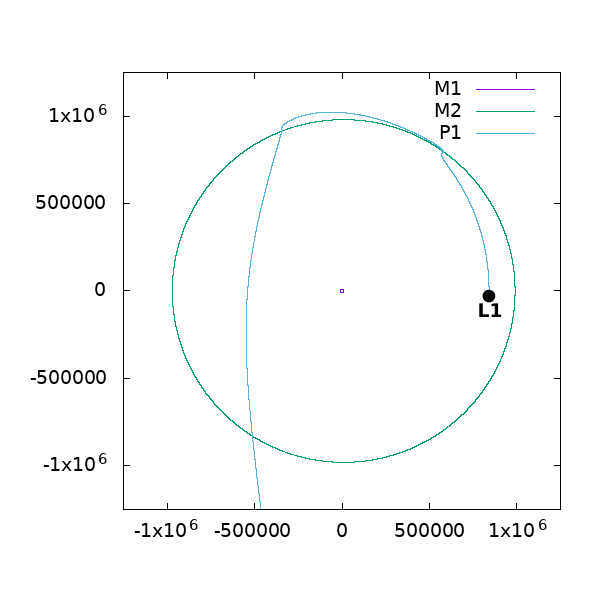
\includegraphics[width = 3 in]{./sim/L1-final.png}
\caption{O ponto grafado como L1 é a posição do ponto de Lagrange 1 no instante inicial. Trata-se de um ponto instável.}
\end{figure}

\begin{figure}[!H]
\centering
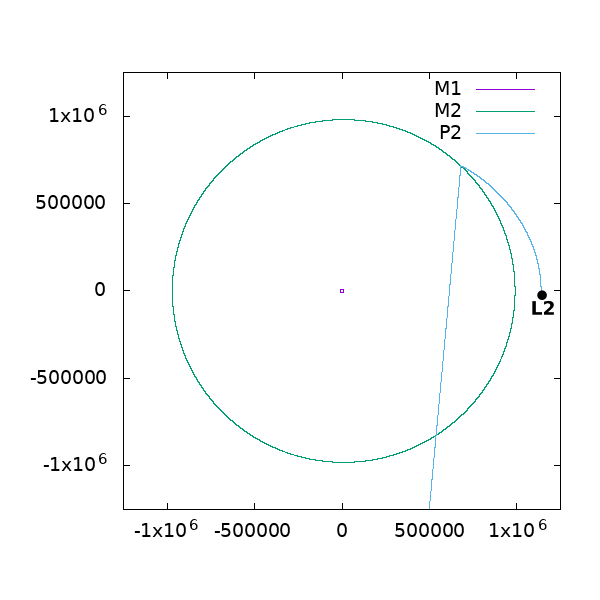
\includegraphics[width = 3 in]{./sim/L2-final.png}
\caption{O ponto grafado como L2 é a posição do ponto de Lagrange 2 no instante inicial. Trata-se de um ponto instável.}
\end{figure}

\begin{figure}[!H]
\centering
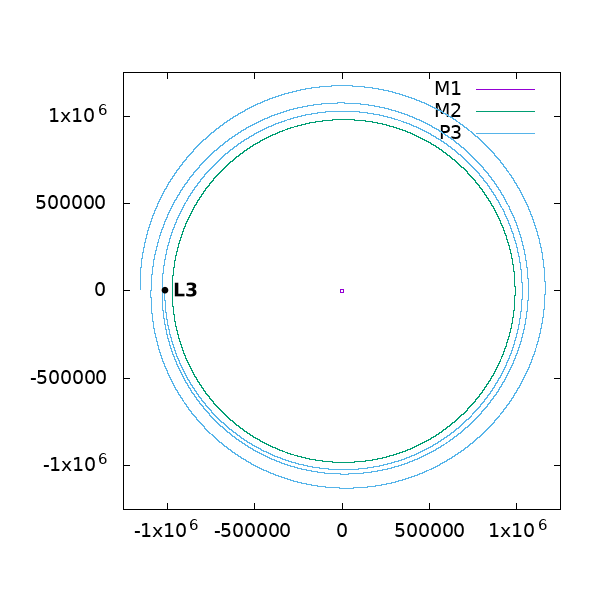
\includegraphics[width = 3 in]{./sim/L3-final.png}
\caption{O ponto grafado como L3 é a posição do ponto de Lagrange 3 no instante inicial. Trata-se de um ponto instável.}
\end{figure}

\begin{figure}[!H]
\centering
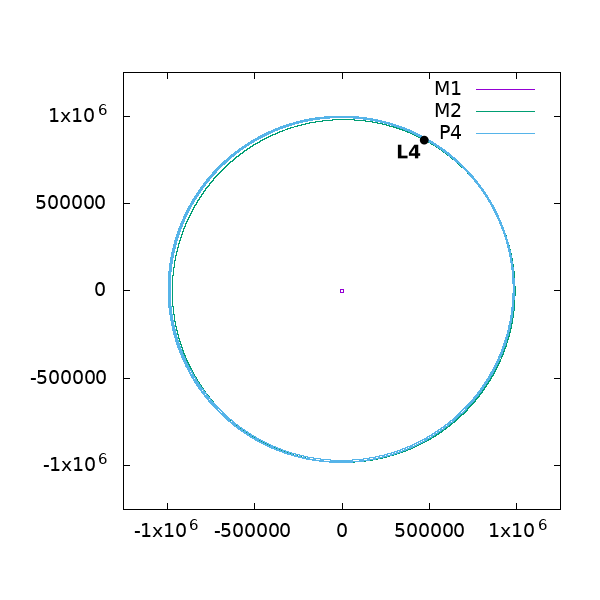
\includegraphics[width = 3 in]{./sim/L4-final.png}
\caption{O ponto grafado como L4 é a posição do ponto de Lagrange 4 no instante inicial. Trata-se, nesse caso, de um ponto estável.}
\end{figure}

\begin{figure}[!H]
\centering
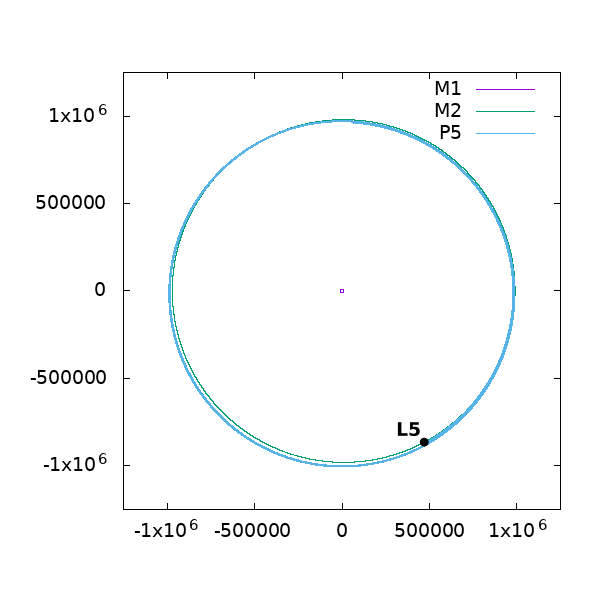
\includegraphics[width = 3 in]{./sim/L5-final.png}
\caption{O ponto grafado como L5 é a posição do ponto de Lagrange 5 no instante inicial. Analogamente a L4, temos para esse caso um ponto estável.}
\end{figure}

   A instabilidade de L1, L2 e L3 é evidenciada pela trajetória descrita pelo terceiro corpo. Ao ser acelerado pelo efeito estilingue, ele se desvia de sua órbita. Por outro lado, em L4 e L5, podemos observar órbitas bem comportadas, o que configura a estabilidade dos pontos.


   \chapter{Conclusão}
      Placeholder


	 \nocite{mccann}\nocite{cornish}
   \bibliography{bib/general.bib}
\end{document}
